\documentclass[dissertation.tex]{subfiles} 
\begin{document}

\chapter{Overview of the Standard Model of Particle Physics}
\label{chap:Overview of the Standard Model of Particle Physics}

%\chapter{The Current State of the Standard Model}

%I call it...the Aristocrats.

%The Standard Model of particle physics describes the elementary building blocks of matter as a set of interacting field quanta.  There are four forces by which the quanta, or particles, may interact: the the weak force, electromagnetic force, the strong force, and the gravitational force.  Table 1 lists some properties of the four forces.

%insert table here showing each force, its carrier, and the physical phenomena it applies to
%\begin{tabular}{|l|l|l|}
%\hline
%Force & Associated particle(s) & Physical phenomena \\
%\hline
%\hline
%Weak & $W^{\pm}$ (80.4 $GeV/c$), $Z^{0}$ (91.2 $GeV/c$) & Radioactive $\beta$ decay, fusion in stars \\
%\hline
%Electromagnetic & Photon & Electricity, 
%\end{tabular}

%In addition to the matter particles, there also exist particles associated to each of the forces.  Interactions between matter particles, for instance via scattering or pair production, are mediated by the exchange or creation of virtual force carriers \cite{Cottingham_and_Greenwood}.

In the 1960s, Sheldon Glashow, Steven Weinberg, and Abdus Salam proposed a mathematical framework that unified the electromagnetic and weak forces at an energy scale in the hundreds of GeV/c, as well as a mechanism for breaking the electroweak symmetry at low energies \cite{Glashow_Weinberg_and_Salam}.  At the same time, Murray Gell-Mann introduced the concept of quarks to describe hadron spectroscopy, a concept that would later grow into quantum chromodynamics (QCD), the full theory of the strong force \cite{Gell-Mann}.  These two key developments motivated the unified representation of particle physics as a set of fields whose dynamics are invariant under the Standard Model gauge group

\begin{equation}
SU(3)_{C} \otimes SU(2)_{L} \otimes U(1)_{EM}
\end{equation}
%        how to make the before-equation spacing equal to the after-equation spacing?
where $SU(3)_{C}$ describes the quark QCD interactions, $SU(2)_{L}$ describes the weak interactions among quarks and leptons, and $U(1)_{EM}$ describes the electromagnetic interaction.

The Standard Model, in particular the electroweak theory, has been an extremely successful predictor of particle production and interaction cross-sections and decay rates, as well as of the exact masses of the electroweak force carriers.  The case for the validity of the Standard Model was bolstered by the many precision QCD and electroweak measurements carried out at the Large Electron-Positron (LEP) collider, which ran from 1989-2000 at center-of-mass energies between 65 and 104 GeV/c \cite{Drees}.  Figure~\ref{fig:LEP} shows some of the highlights of the LEP program.

\begin{figure}
	\centering
	\subfloat[Total hadronic cross-section as a function of collider center-of-mass energy.]{\label{fig:LEP_hadronic_xsec}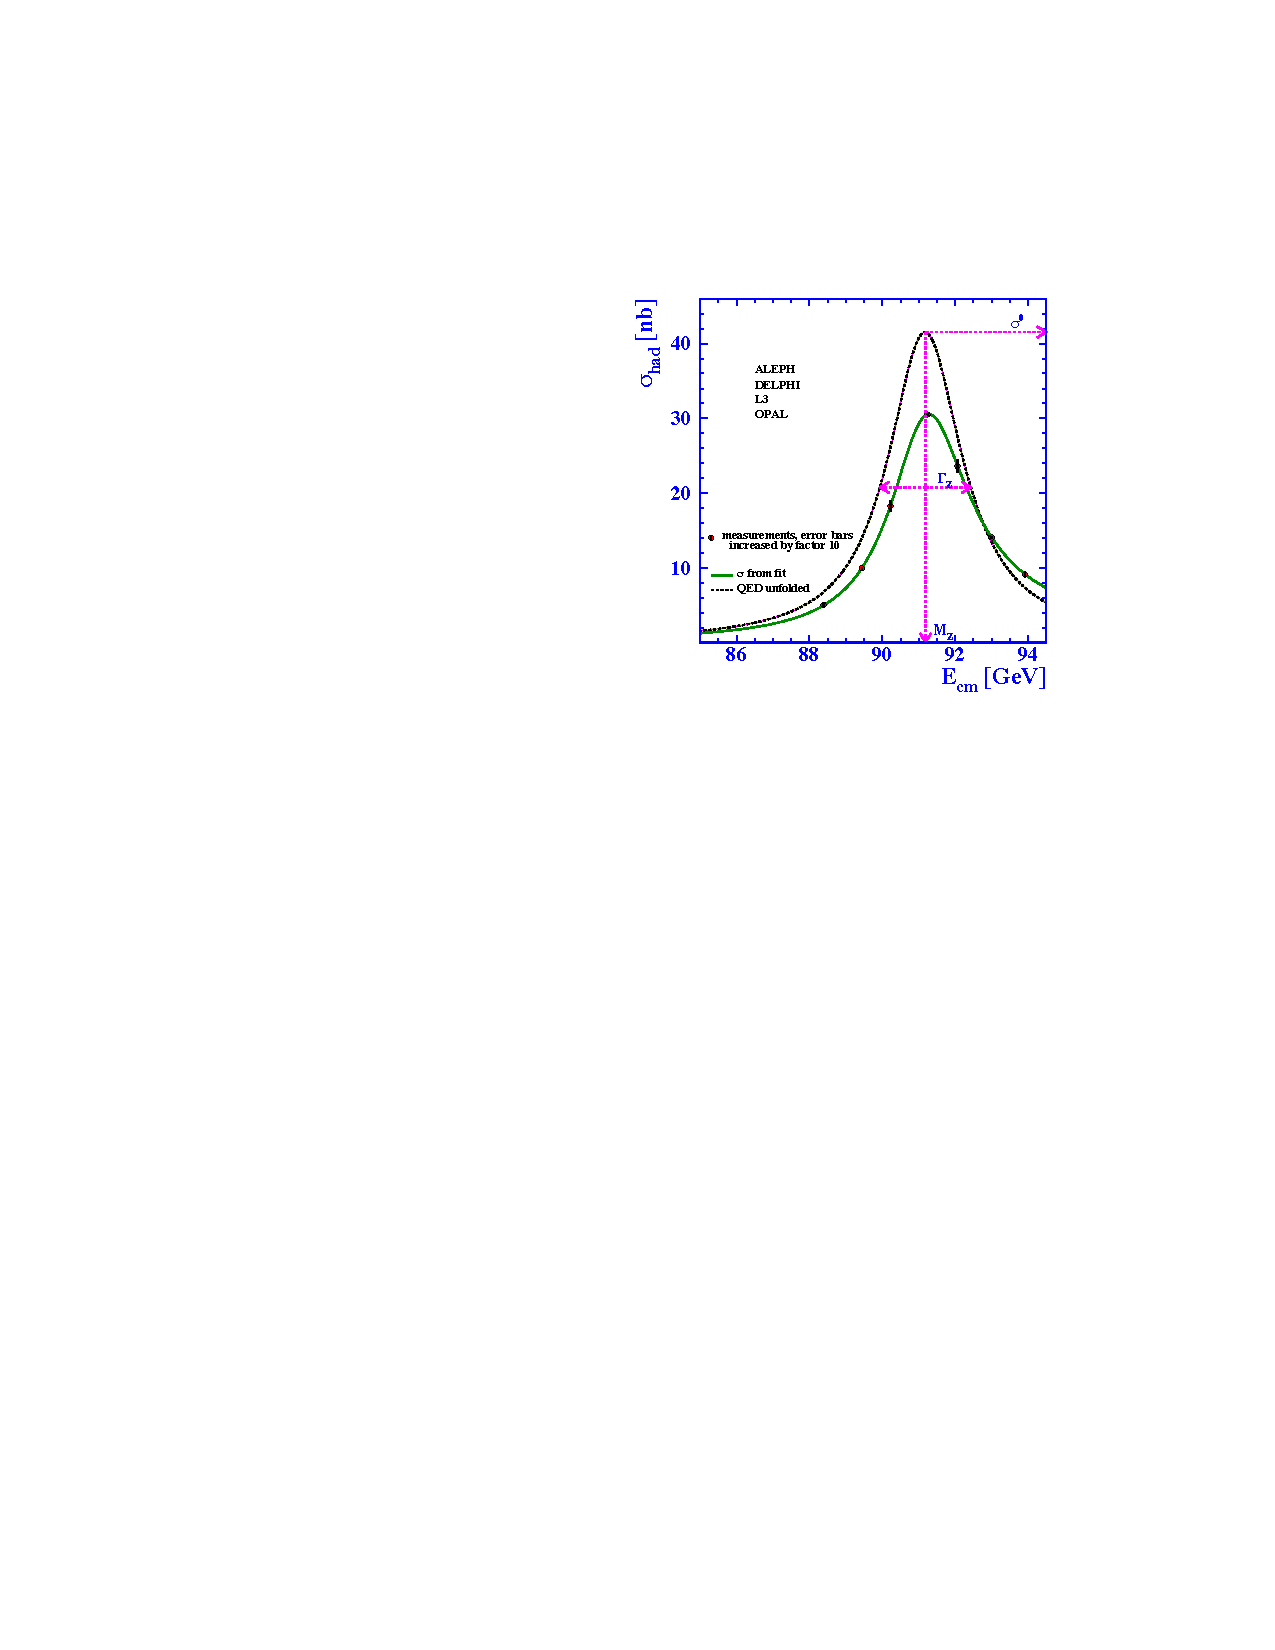
\includegraphics[scale=0.7]{LEP_hadronic_xsec}}
	\hspace{1cm}
	\subfloat[Measured and predicted dependence of the $q\overline{q}$, $\mu^{+}\mu^{-}$, and $\tau^{+}\tau^{-}$ pair production cross sections on LEP center-of-mass energy.]{\label{fig:LEP_pair_production_xsecs}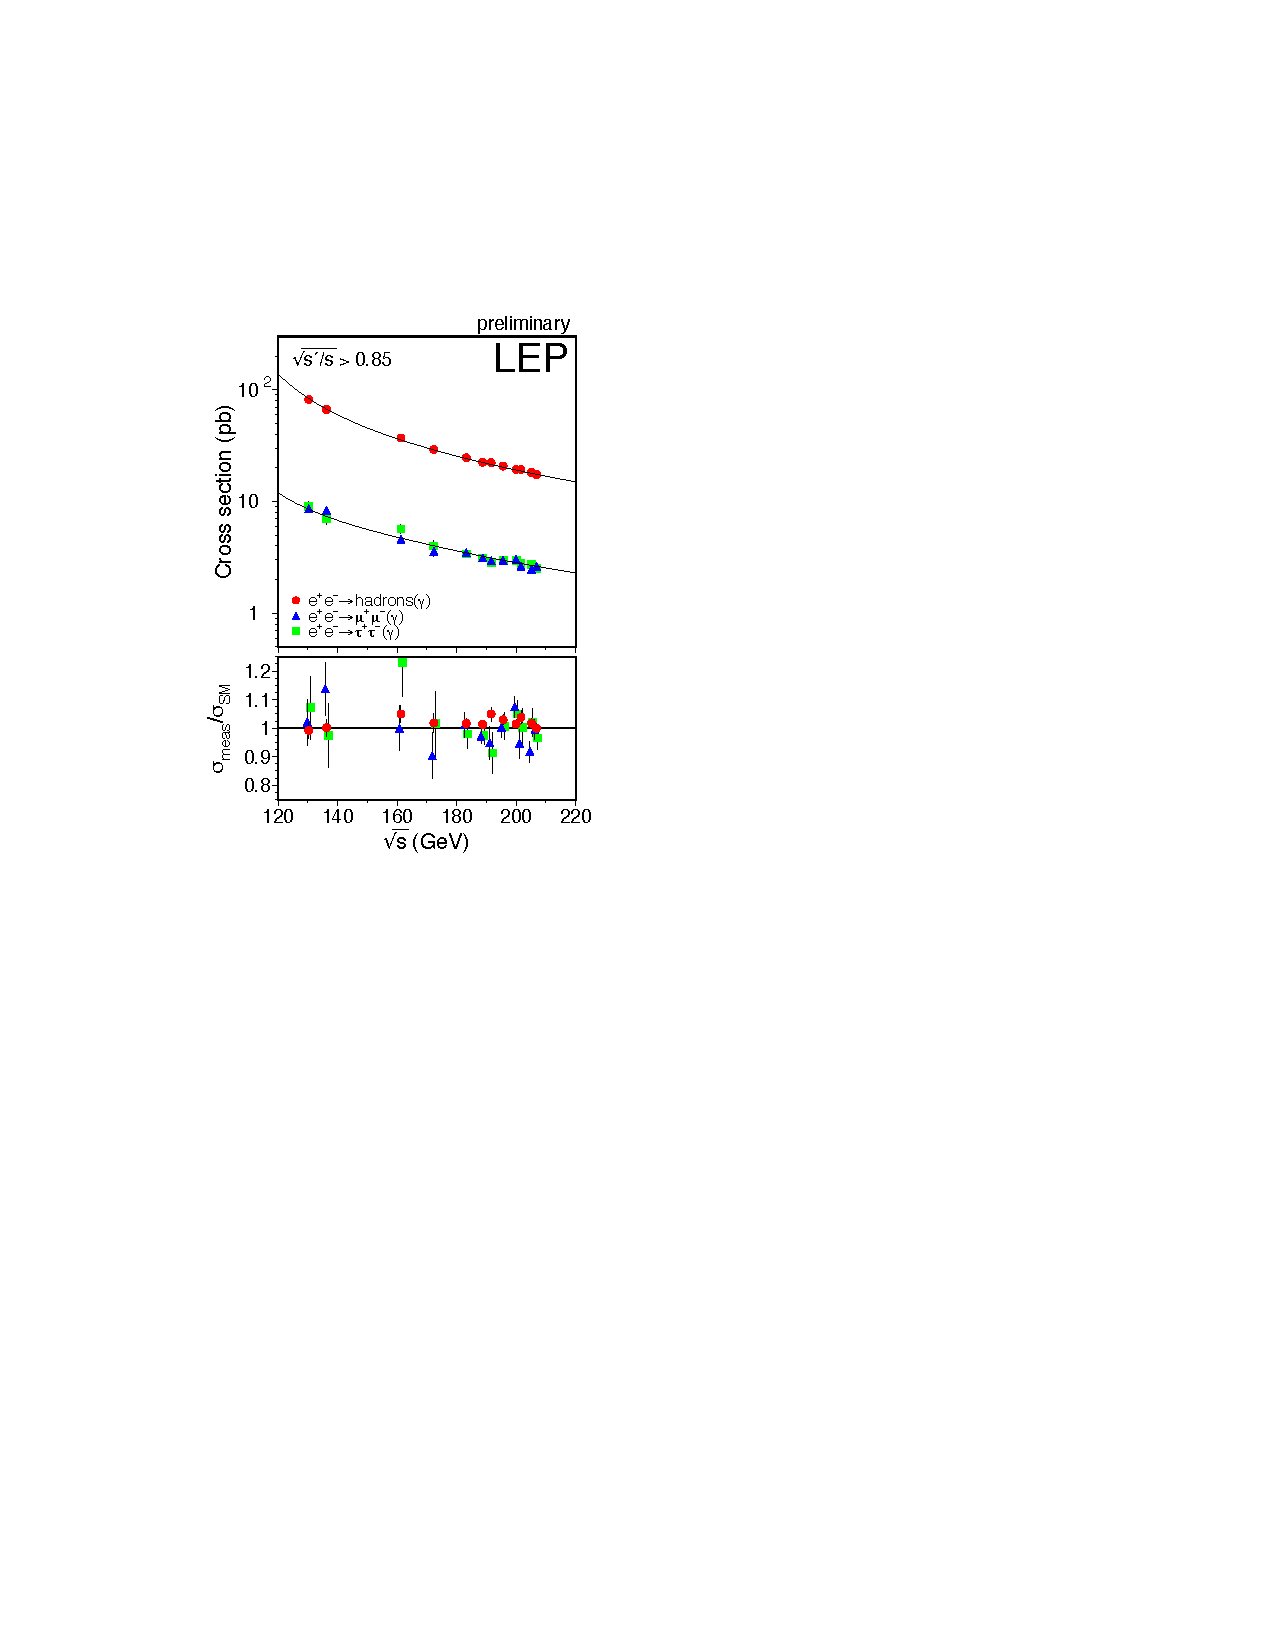
\includegraphics[scale=0.7]{LEP_pair_production_xsecs}}
	\\
	\subfloat[Measured and predicted dependence of the $W^{+}W^{-}$ pair production cross section on LEP center-of-mass energy.]{\label{fig:LEP_W_pair_production_xsec}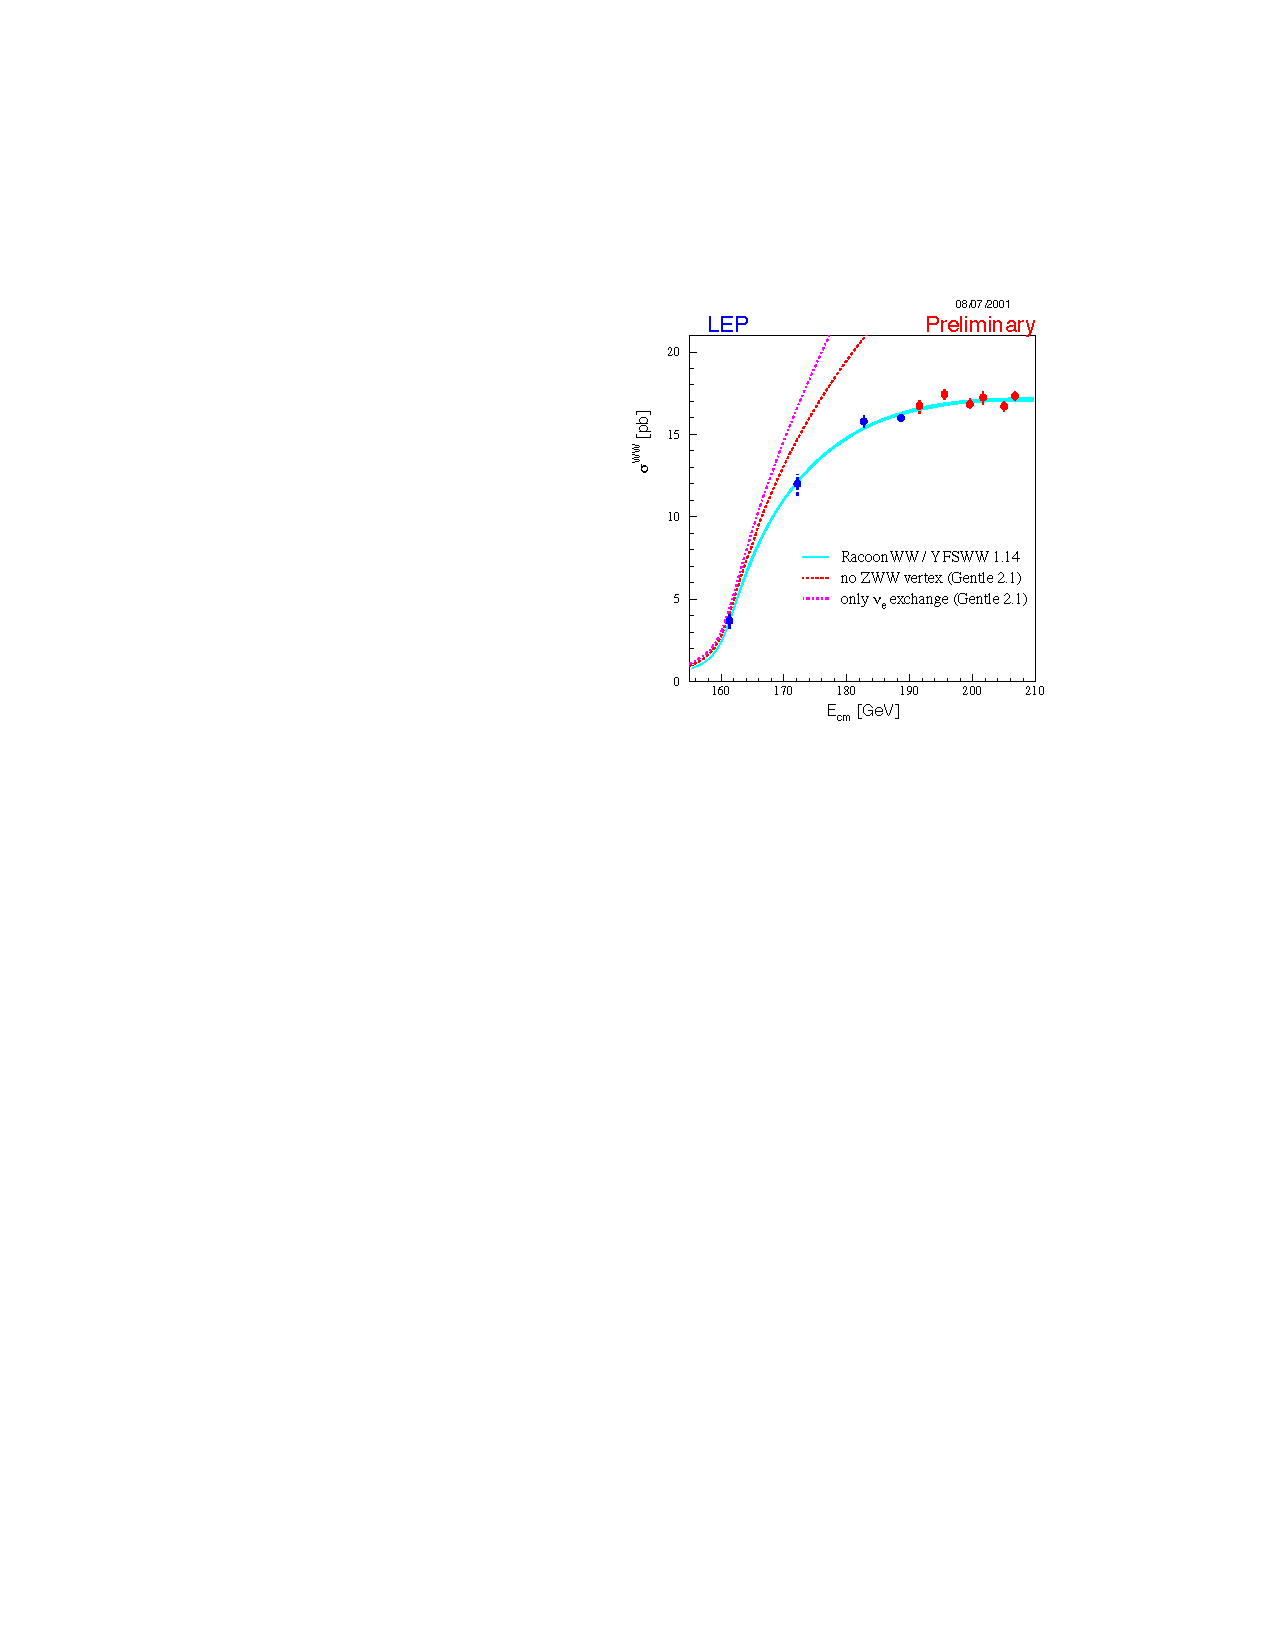
\includegraphics[scale=0.7]{LEP_W_pair_production_xsec}}
	\hspace{1cm}
	\subfloat[Measured and predicted dependence of the strong coupling constant $\alpha_{s}$ on LEP center-of-mass energy.]{\label{fig:LEP_alphaS_running}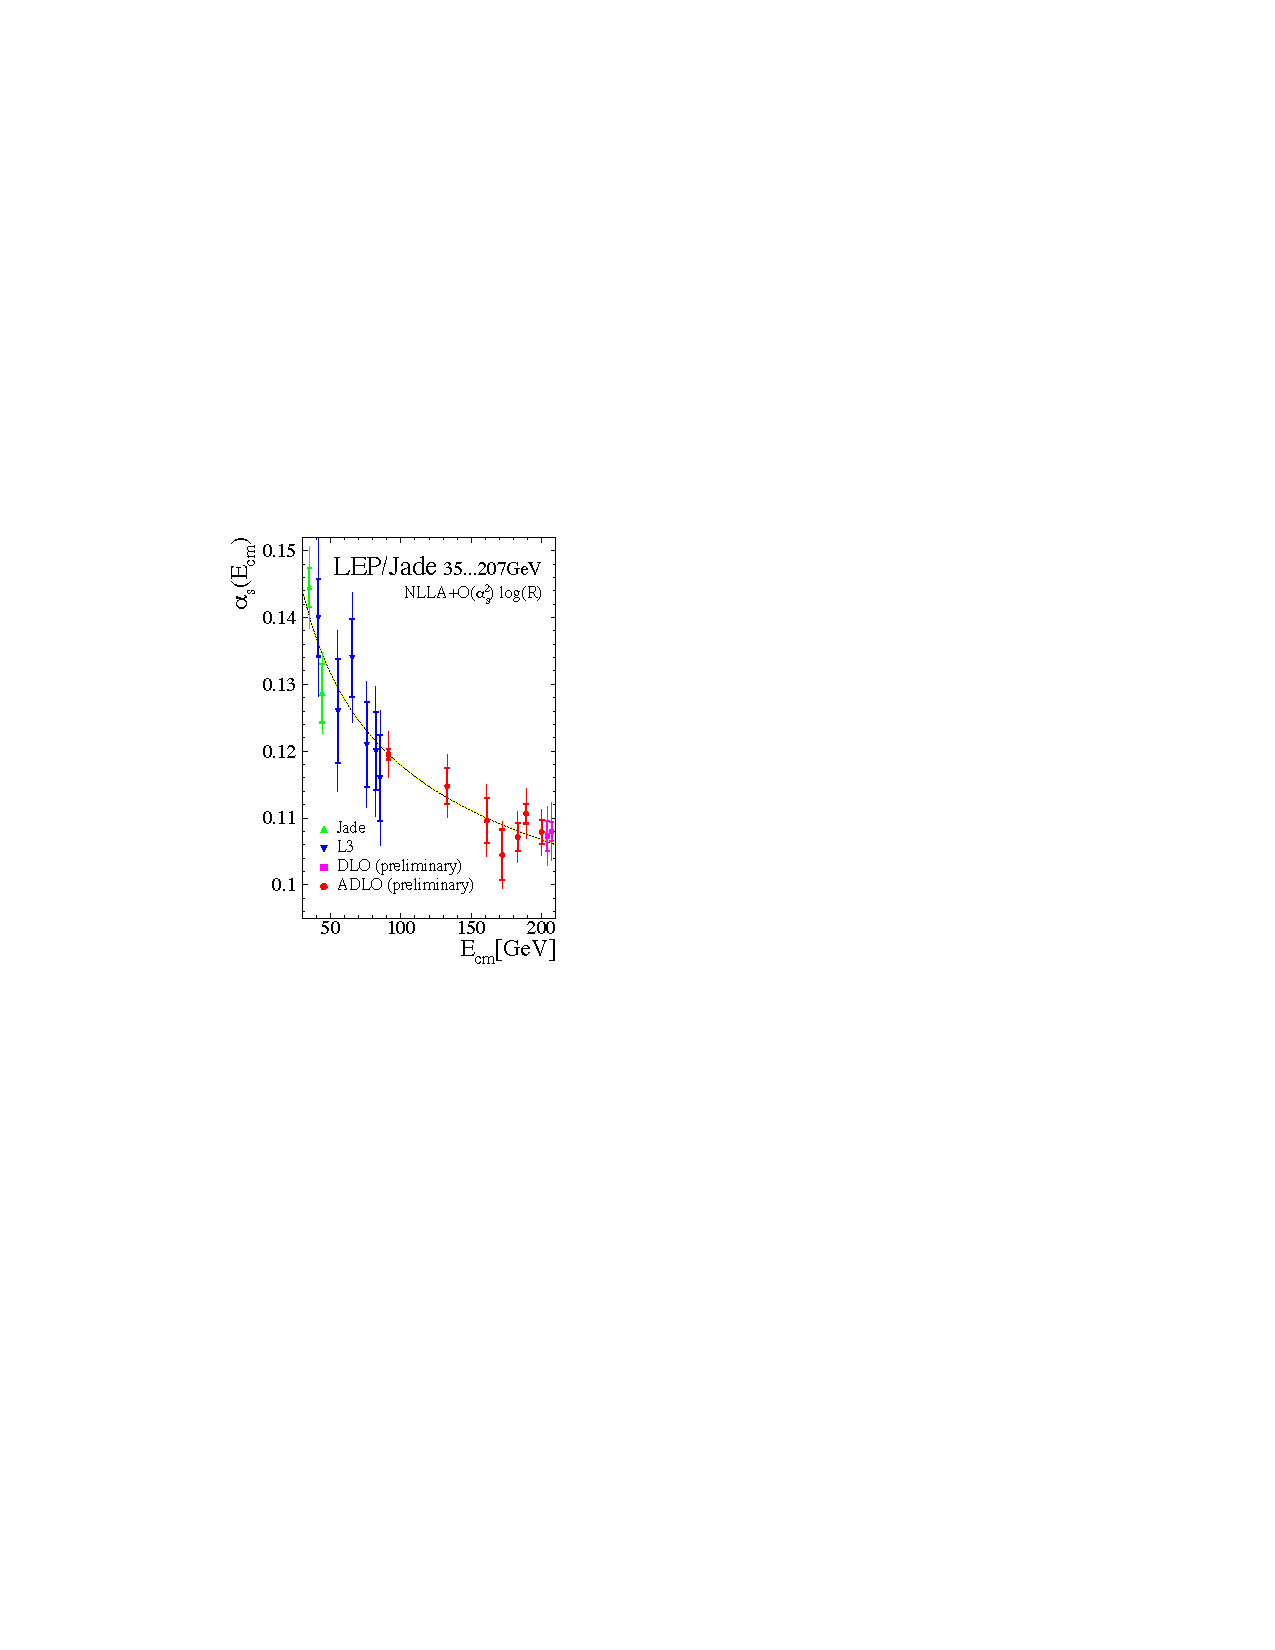
\includegraphics[scale=0.7]{LEP_alphaS_running}}
	\caption{Selected LEP measurements demonstrating its contribution to the precise understanding of the Standard Model.  Reprinted from \cite{Drees}.}
	\label{fig:LEP}
\end{figure}

However, there are still deep theoretical problems with the Standard Model, stemming from the introduction of the Higgs scalar into the theory to break electroweak symmetry \cite{Higgs}.  Since the Higgs self-energy diagram is quadratically sensitive to the ultraviolet cutoff scale(footnote: this is a general property of scalar fields), and assuming that there are no new important energy scales of physics between the weak scale ($\mathcal{O}$($10^{2}$ GeV/c)) and the Planck scale ($\mathcal{O}$($10^{19}$ GeV/c)), in order to be consistent with experimental measurements, this diagram must include a remarkable 17-orders-of-magnitude cancellation that is otherwise poorly motivated \cite{Aitchison}.  The quest to find new physics at an intermediate energy scale between the weak and Planck scales, and thus extend the Standard Model, was the driving force behind the construction of the Large Hadron Collider (LHC) in 2009, the world's highest energy particle accelerator to date.

In this chapter I will briefly describe the Standard Model particle content, the theory and major results of electroweak symmetry breaking (EWSB), and the problems that the Standard Model is as yet ill-prepared to address.

\section{Particle Content}
%group theory representation
%doublets, singlets, charges
%masses: why so different?
%Fermi vs. Bose statistics
\section{Electroweak Symmetry Breaking and the Higgs Mechanism}
\section{The Hierarchy Problem, The Origins of Mass, and Fine Tuning}
%show how SUSY makes mu^2 negative
%show how SUSY unifies the coupling constants

\end{document}